\documentclass[11pt,a4paper]{article}
\usepackage{fontspec}
\setmainfont{TeX Gyre Pagella}
\newfontfamily\headfont{Inter}[UprightFont=*-ExtraBold,BoldFont=*-ExtraBold,Extension=.otf,Path=/usr/share/fonts/opentype/inter/]
\usepackage[a4paper,margin=2.3cm]{geometry}
\usepackage{graphicx,booktabs,float,caption,array,xcolor}
\usepackage[hidelinks]{hyperref}
\usepackage{titlesec}
\usepackage[round]{natbib}
\usepackage{setspace}
\setstretch{1.05}
\renewcommand{\topfraction}{0.9}
\renewcommand{\bottomfraction}{0.8}
\renewcommand{\textfraction}{0.1}
\renewcommand{\floatpagefraction}{0.75}
\setlength{\parindent}{0pt}
\setlength{\parskip}{0.55em}
\titleformat{\section}{\headfont\Large}{\thesection}{0.8em}{}
\titleformat{\subsection}{\headfont\large}{\thesubsection}{0.8em}{}
\captionsetup{font=small,labelfont=bf}
\urlstyle{same}
\hypersetup{pdftitle={In the Shadow of the Volcano: How Many People Live Near the World's Holocene Volcanoes},pdfauthor={Tristan Hotham}}

\begin{document}
\begin{center}
{\Large\bfseries In the Shadow of the Volcano\par}
\vspace{0.4em}
{\large How many people live near the world's Holocene volcanoes,\\from the Smithsonian's Volcanoes of the World database\par}
\vspace{1.2em}
{\large Tristan Hotham\par}
\vspace{0.3em}
{\small Independent researcher\\
ORCID: 0000-0003-4931-9349\\
DOI: \href{https://doi.org/10.5281/zenodo.23847550}{https://doi.org/10.5281/zenodo.23847550}\par}
\vspace{0.8em}
2026
\end{center}

\begin{quote}
\small
\begin{center}\textbf{Abstract}\end{center}
The Smithsonian Institution's Global Volcanism Program (GVP) lists 1,215 volcanoes with evidence of activity in the Holocene and gives, for most of them, the number of people living within 5, 10, 30 and 100 km. Summing those figures counts people who live near several volcanoes more than once. I bound the number of distinct people from below by summing only volcanoes whose circles do not overlap, and from above by the simple sum. At least 52.9 million people live within 10 km of a Holocene volcano (upper bound 56.4 million), at least 147.5 million within 30 km (upper bound 273.5 million) and at least 532.4 million within 100 km. Indonesia accounts for 28\% of the 30 km lower bound, followed by Mexico, Japan, the Philippines and Italy. 76 volcanoes have a million or more people within 30 km; the most crowded are the Tatun Volcanic Group beside Taipei, the Michoac\'an-Guanajuato field in Mexico and Tangkuban Parahu above Bandung. 21 volcanoes with a million or more people within 30 km have erupted since 2000. Recorded eruptions rise 8.8-fold from the seventeenth to the twentieth century while eruptions of VEI 4 or more rise 2.0-fold, a pattern that reflects reporting more than volcanism. The population figures are a fixed snapshot from the GVP and the distances are not hazard zones.

\textbf{Keywords:} volcanoes; population exposure; Holocene; Global Volcanism Program; Volcanoes of the World; Ring of Fire; reporting bias; mapping
\end{quote}

\section{Introduction}
Volcanoes attract people. Volcanic soils are fertile, volcanic highlands are cooler and wetter than the lowlands around them, and many volcanic arcs are also the backbones of densely settled islands and isthmuses. The result is that some of the world's large cities, from Naples to Mexico City, Manila, Jakarta, Bandung and Taipei, lie within a short distance of a volcano that has erupted in the last 12,000 years.

The reference list of those volcanoes is kept by the Smithsonian Institution's Global Volcanism Program in its database Volcanoes of the World \citep{gvp535}. For each Holocene volcano it records the location, type, elevation, tectonic setting and last known eruption, and it publishes a separate list of dated eruptions. It has also published, for each volcano, the number of people living within 5, 10, 30 and 100 km. Earlier work used figures of this kind to describe the populations exposed to volcanoes worldwide and to build a population exposure index \citep{brown2015}.

This paper is a descriptive companion to an interactive map (\url{https://maps.tristanhotham.com/volcano-neighbours/}). It asks four questions of the GVP data: how many people live near a Holocene volcano, counted so that no one is counted twice; in which countries; near which volcanoes; and how many of those volcanoes have erupted recently. It also looks at the eruption record over time, which says as much about who was watching as about what volcanoes did.

\section{Data}
\subsection{Volcano and eruption lists}
The volcano list is the GVP Holocene volcano list from Volcanoes of the World version 5.3.5 \citep{gvp535}, an export whose header records that it was downloaded in 2026. It holds 1,215 volcanoes in 77 countries and territories (a volcano on a border is listed under both countries; 165 are in the United States, 118 in Japan and 101 in Indonesia). The eruption list is the GVP list of confirmed Holocene eruptions from the same version, also downloaded in 2026: 9,918 eruptions at 849 volcanoes, with start dates, the Volcanic Explosivity Index (VEI; \citealt{newhall1982}) where known (78\% of eruptions) and the method used to date each eruption. I used copies of both exports posted to public GitHub repositories, identified by their headers; their sources are listed under Data availability.

The GVP records a volcano's last known eruption. For a long eruption this is the date it ended, and for one still continuing it is the current year, so it can be later than the start of the most recent eruption in the eruption list (145 volcanoes). 366 volcanoes have no dated eruption: they are on the list because of other evidence of Holocene activity, such as young lava flows or thermal features.

\subsection{Population figures}
The GVP's current exports no longer carry the population columns, so I took them from a copy of the volcano list from version 5.1.7 \citep{gvp517}, which does, and joined them by volcano number. Of the 1,215 volcanoes in version 5.3.5, 1,209 have population figures; the 6 without are volcanoes added or renumbered since. The figures are identical to those in a GVP export used by the TidyTuesday project in 2020, so they are a fixed snapshot rather than a series that is updated with each version. The export does not say which population grid or reference year they come from; they should be read as an estimate for the early part of the last decade and are likely to understate today's populations in fast-growing places.

For 16 volcanoes, most of them large volcanic fields, the GVP gives the same figure at 10 and 30 km. The Michoac\'an-Guanajuato field in Mexico, for example, has 5,783,287 people at every distance from 5 to 100 km. This suggests that for these fields the count covers the whole field rather than circles around its listed point. I keep the GVP's figures and flag these cases.

\subsection{Other sources}
Deaths come from the NOAA NCEI Global Significant Volcanic Eruptions Database \citep{ncei}, using a copy made in 2024 that holds the 442 eruptions with deaths recorded. Plate boundaries are the PB2002 model of \citet{bird2003}. Country outlines and city names are from Natural Earth \citep{naturalearth}.

\section{Methods}
\textbf{Bounds on the number of people.} Let $P_i(r)$ be the population within $r$ km of volcano $i$. The simple sum $\sum_i P_i(r)$ is an upper bound on the number of distinct people within $r$ km of at least one volcano: each such person is counted at least once, and some several times. For a lower bound, I sort volcanoes by $P_i(r)$ in descending order and keep a volcano if its distance to every volcano already kept is more than $2r$, so that their circles cannot overlap. The populations of kept volcanoes are populations of disjoint areas, so their sum is a true lower bound. The greedy choice keeps the most crowded volcano in each cluster; it is not the best possible lower bound, but it is simple, transparent and close to the upper bound wherever circles rarely overlap. Distances are great-circle distances between the GVP's listed points. The same method is applied within each country and within each group of volcanoes by date of last eruption.

\textbf{Countries.} A volcano is assigned to every country in its GVP country field, so that a volcano on the border of Chile and Argentina counts for both. Populations are those around the volcano and can include people across a border.

\textbf{Eruptions over time.} Confirmed eruptions are counted by century of their start year, and separately for eruptions of VEI 4 or more. The final century covers only 2000 to 2026 (27 years).

\section{Results}
\subsection{How many people live near a Holocene volcano}
Table~\ref{tab:bounds} and Figure~\ref{fig:bounds} give the bounds. Within 5 and 10 km the circles of different volcanoes rarely overlap and the two bounds are close: between 52.9 million and 56.4 million people live within 10 km of a Holocene volcano. At 30 km the bounds are 147.5 million and 273.5 million. At 100 km circles overlap so much (1,131 of the 1,209 volcanoes have another volcano within 200 km) that the simple sum, 2.5 billion, is far too high; the lower bound is 532.4 million, and \citet{brown2015}, counting people on a population grid, report a figure of roughly 800 million, between the two.

\begin{table}[tbp]\centering\footnotesize\setlength{\tabcolsep}{4pt}\caption{People near Holocene volcanoes: lower bound (sum over non-overlapping circles, with the number of volcanoes kept), upper bound (simple sum over all 1,209 volcanoes with figures) and the number of volcanoes with nobody within the distance.}\label{tab:bounds}\begin{tabular}{lrrrr}\toprule Distance & Lower bound & Volcanoes kept & Upper bound & Volcanoes with nobody\\\midrule
Within 5 km & 42,056,128 & 742 & 42,196,972 & 436\\
Within 10 km & 52,937,756 & 716 & 56,424,613 & 357\\
Within 30 km & 147,481,561 & 490 & 273,543,823 & 247\\
Within 100 km & 532,377,057 & 245 & 2,466,043,644 & 151\\
\bottomrule\end{tabular}\end{table}

\begin{figure}[tbp]\centering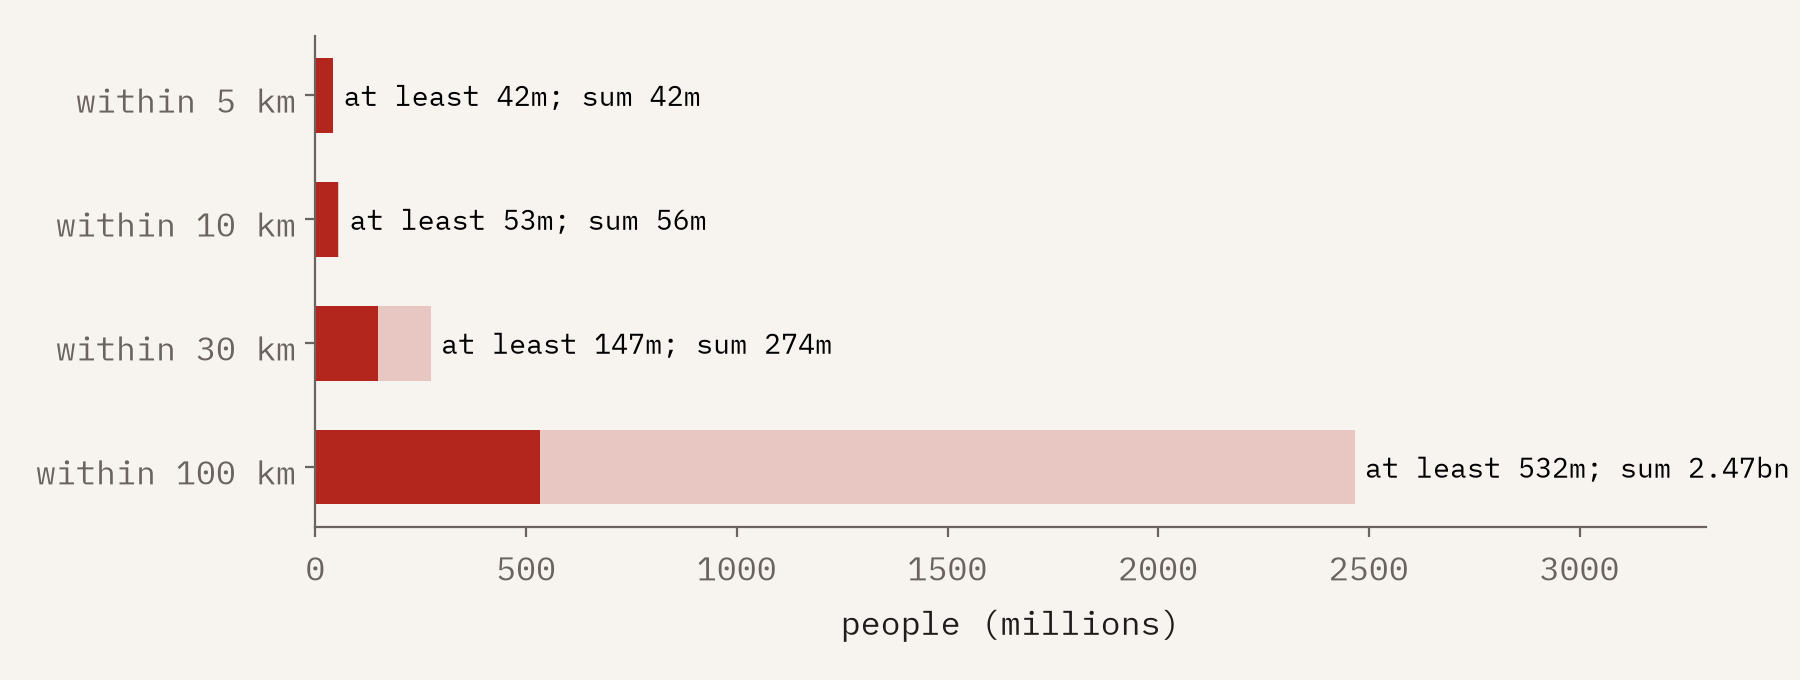
\includegraphics[width=.86\textwidth]{f_bounds.png}
\caption{People within 5, 10, 30 and 100 km of a Holocene volcano. Solid: lower bound (non-overlapping circles). Pale: simple sum over volcanoes (upper bound).}\label{fig:bounds}\end{figure}

Most volcanoes have few neighbours. 357 of the 1,209 volcanoes with figures (30\%) have nobody within 10 km and the median volcano has 4,732 people within 30 km. The distribution is very skewed: the 20 most crowded volcanoes hold 27\% of the 30 km sum and the 100 most crowded 68\%. 76 volcanoes have at least a million people within 30 km, 94 have at least 100,000 within 10 km, and 49 have at least ten million within 100 km. Stratovolcanoes, the classic steep cones, make up 551 of the list and 49\% of the 30 km sum; volcanoes in subduction zones account for 86\% of it. Figure~\ref{fig:map} maps the volcanoes by population within 30 km and date of last eruption, with the plate boundaries that outline the Pacific Ring of Fire.

\begin{figure}[tbp]\centering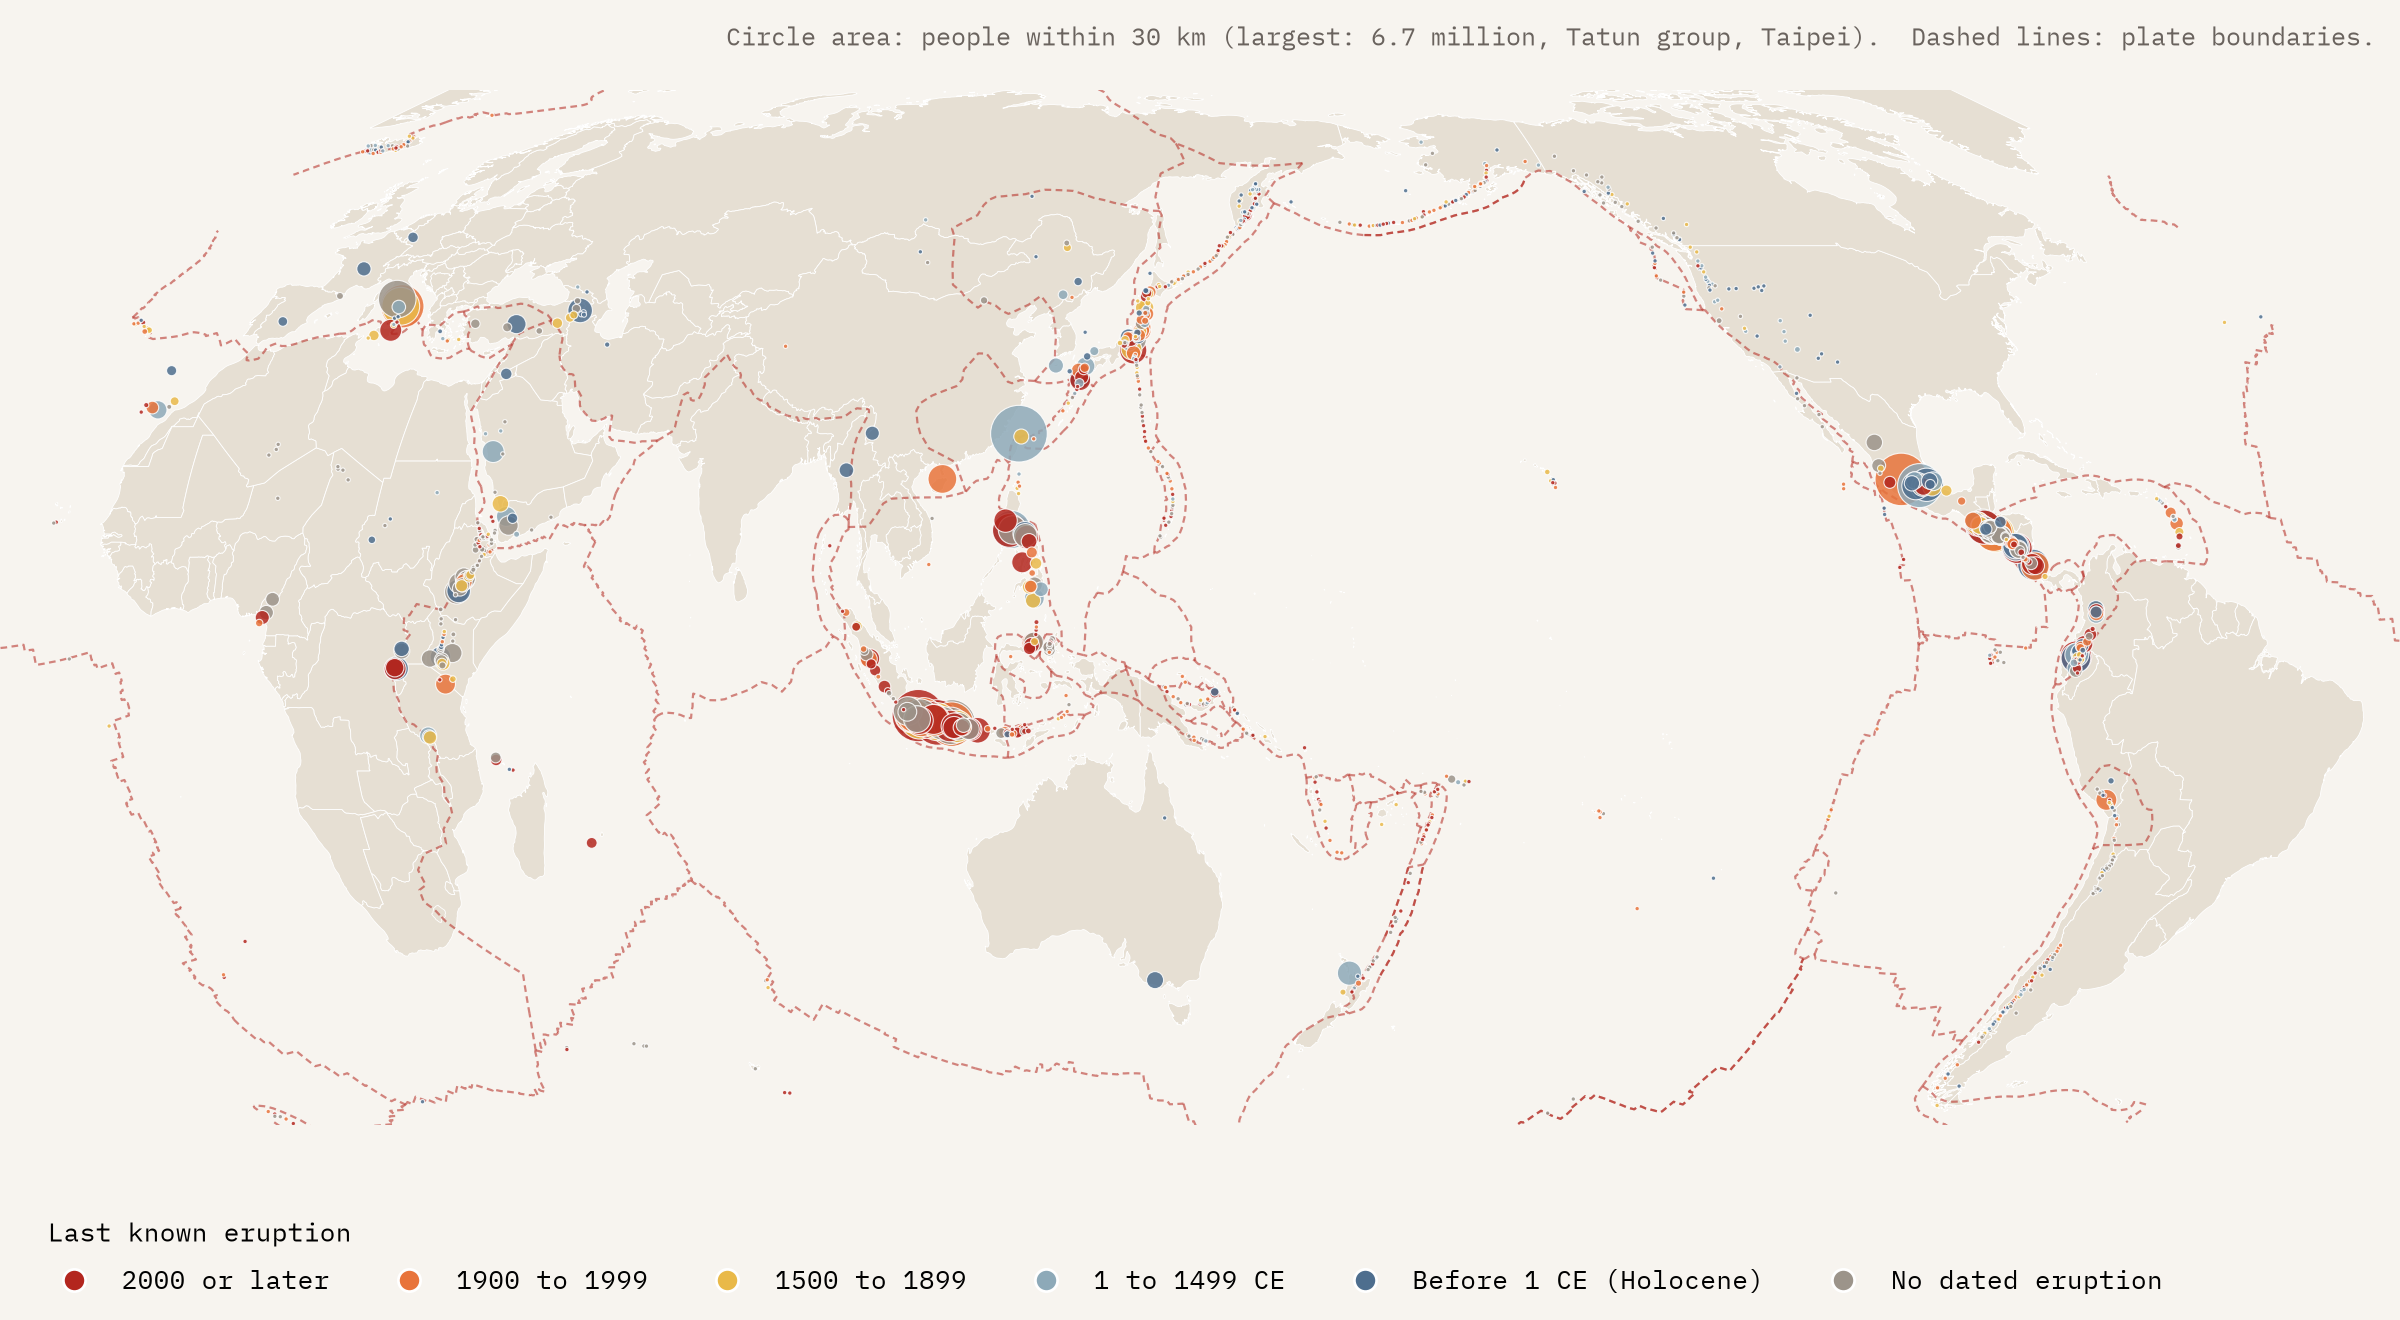
\includegraphics[width=\textwidth]{f_map.png}
\caption{Holocene volcanoes, sized by population within 30 km and coloured by last known eruption, on a Pacific-centred Equal Earth projection. Dashed lines: plate boundaries \citep{bird2003}.}\label{fig:map}\end{figure}

\subsection{Countries}
Indonesia stands out (Table~\ref{tab:countries}, Figure~\ref{fig:countries}). It has 101 Holocene volcanoes, 40 of which have erupted since 2000, and at least 41.8 million people within 30 km of one (28\% of the world's lower bound) and 120.3 million within 100 km. Mexico (18.7 million), Japan (10.1 million), the Philippines (9.7 million) and Italy (8.2 million) follow, and together the top five hold 60\% of the world lower bound. Taiwan ranks sixth with only 2 volcanoes, because one is on the edge of Taipei. In Central America the upper and lower bounds differ most: El Salvador and Guatemala have many volcanoes in a small area, so circles overlap widely. Countries with many volcanoes but few neighbours include the United States (165 volcanoes, at least 549,000 people within 30 km), Russia, Chile and Iceland.

\begin{figure}[tbp]\centering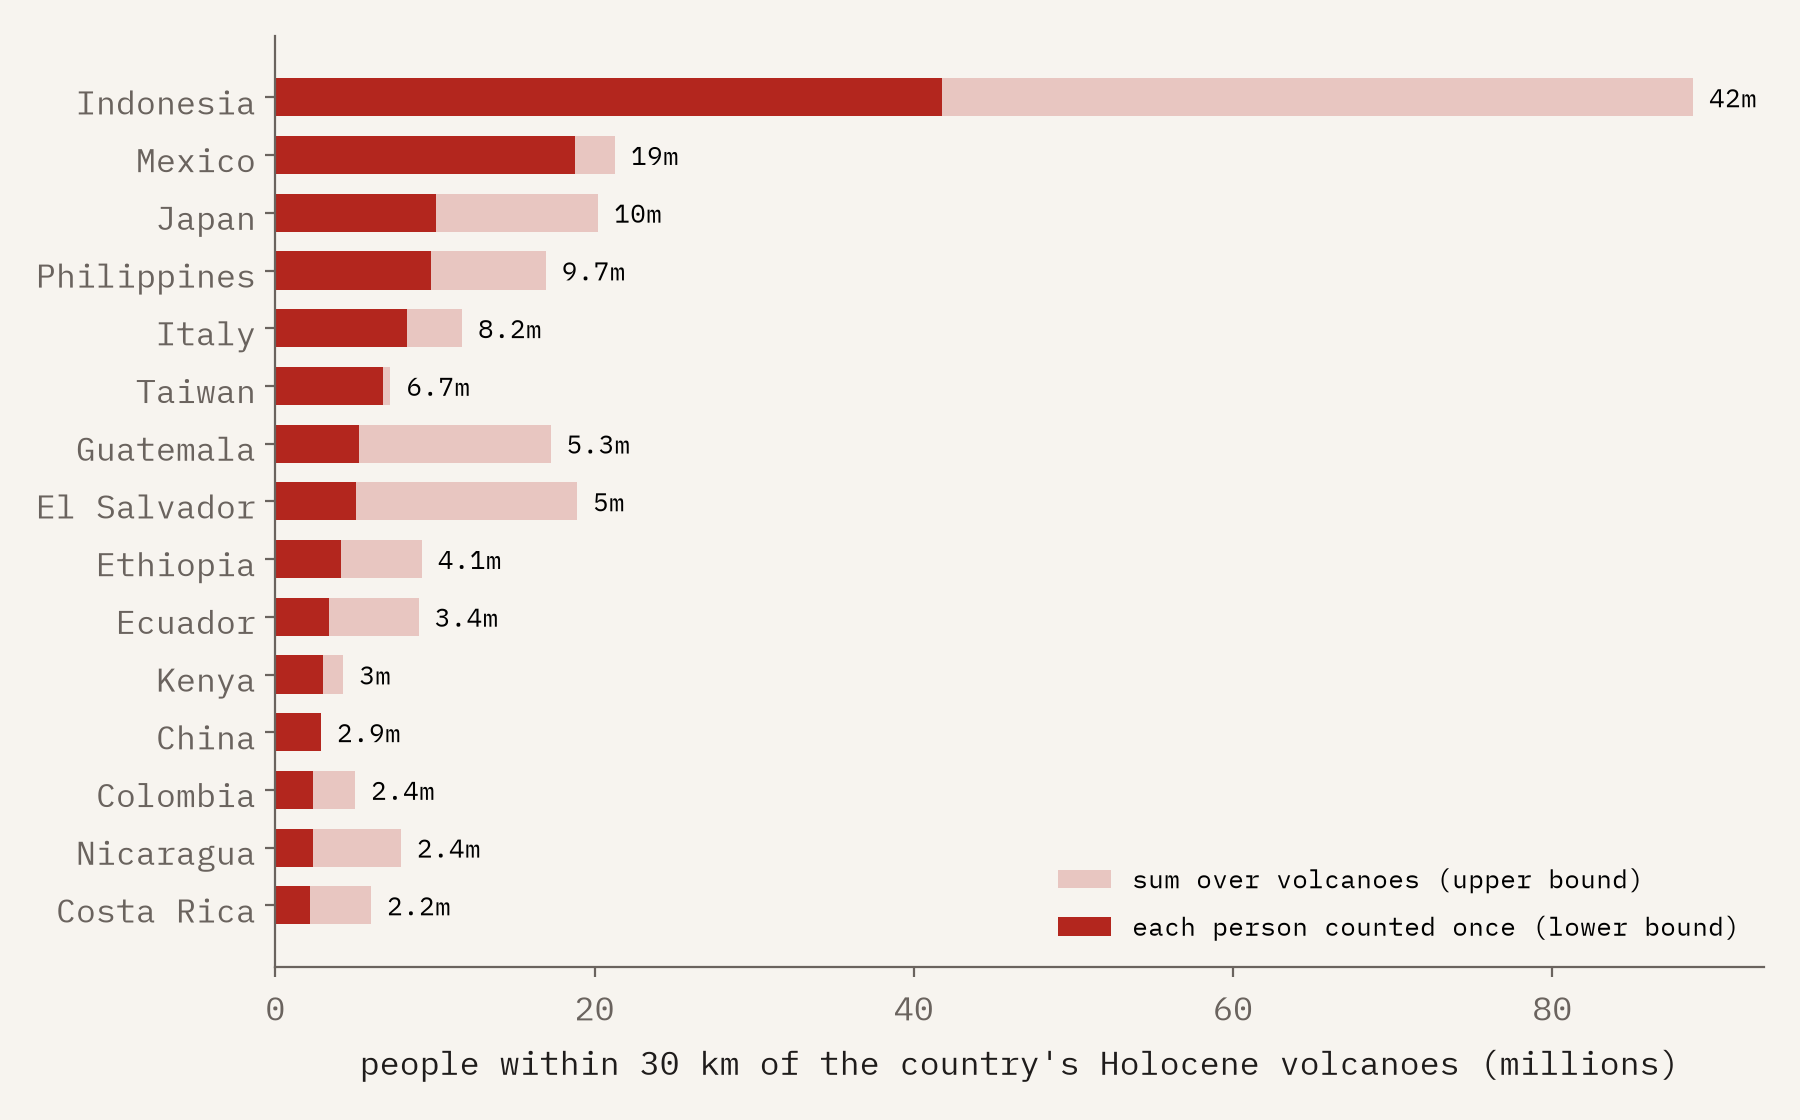
\includegraphics[width=.86\textwidth]{f_countries.png}
\caption{The fifteen countries with most people within 30 km of their Holocene volcanoes: lower bound (solid) and simple sum (pale).}\label{fig:countries}\end{figure}

\begin{table}[tbp]\centering\footnotesize\caption{Countries ranked by the lower bound of people within 30 km of their Holocene volcanoes (millions). Lower bounds (LB) count each person once; the 30 km sum is the upper bound.}\label{tab:countries}\setlength{\tabcolsep}{4pt}\begin{tabular}{lrrrrrrl}\toprule Country & Volcanoes & Since 2000 & LB 10 km & LB 30 km & Sum 30 km & LB 100 km & Most crowded (30 km)\\\midrule
Indonesia & 101 & 40 & 6.3 & 41.8 & 88.8 & 120.3 & Tangkuban Parahu\\
Mexico & 30 & 2 & 7.6 & 18.7 & 21.3 & 50.0 & Michoacan-Guanajuato\\
Japan & 118 & 22 & 1.5 & 10.1 & 20.2 & 65.1 & Hakoneyama\\
Philippines & 23 & 5 & 3.1 & 9.7 & 16.9 & 48.6 & San Pablo Volcanic Field\\
Italy & 13 & 2 & 4.1 & 8.2 & 11.7 & 9.7 & Vesuvius\\
Taiwan & 2 & 0 & 5.1 & 6.7 & 7.2 & 10.0 & Tatun Volcanic Group\\
Guatemala & 20 & 3 & 1.4 & 5.3 & 17.2 & 15.1 & Agua\\
El Salvador & 17 & 2 & 4.4 & 5.0 & 18.9 & 7.2 & Ilopango\\
Ethiopia & 49 & 6 & 2.7 & 4.1 & 9.2 & 22.9 & Bilate River Field\\
Ecuador & 36 & 9 & 1.5 & 3.4 & 9.0 & 6.2 & Guagua Pichincha\\
Kenya & 21 & 0 & 0.6 & 3.0 & 4.2 & 25.0 & Menengai\\
China & 10 & 0 & 2.1 & 2.9 & 2.9 & 20.1 & Hainan Volcanic Field\\
Colombia & 14 & 4 & 0.2 & 2.4 & 5.0 & 10.8 & Galeras\\
Nicaragua & 13 & 5 & 2.1 & 2.4 & 7.9 & 3.6 & Masaya\\
Costa Rica & 10 & 4 & 0.1 & 2.2 & 6.0 & 4.0 & Barva\\
Saudi Arabia & 8 & 0 & 1.6 & 1.9 & 1.9 & 5.0 & Rahat, Harrat\\
Yemen & 10 & 2 & 1.4 & 1.9 & 1.9 & 9.1 & Arhab, Harra of\\
Turkey & 7 & 0 & 0.1 & 1.6 & 1.8 & 11.2 & Erciyes Volcanic Complex\\
Spain & 8 & 2 & 0.4 & 1.6 & 1.6 & 7.4 & Gran Canaria\\
Armenia & 5 & 0 & 1.3 & 1.5 & 1.6 & 3.2 & Ghegham Volcanic Ridge\\
\bottomrule\end{tabular}\end{table}

\subsection{The most crowded volcanoes}
By population within 30 km the most crowded volcanoes are the Tatun Volcanic Group on the northern edge of Taipei (6,735,396), the Michoac\'an-Guanajuato volcanic field in Mexico (5,783,287), Tangkuban Parahu above Bandung (5,729,309), Penanggungan near Surabaya (4,605,710) and Merapi above Yogyakarta (4,348,473) (Table~\ref{tab:top}, Figure~\ref{fig:top}). Vesuvius has 3,907,941 people within 30 km and Campi Flegrei 3,006,865; the two are 24 km apart, and most of Naples falls within 30 km of both, a clear case of the double counting that the lower bound removes. Within 10 km, the leaders are fields and calderas beneath cities: Michoac\'an-Guanajuato, the Tatun group, Campi Flegrei (2,234,109) and Ilopango beside San Salvador (2,049,583). Within 100 km, the Javanese volcanoes near Jakarta lead, Gede-Pangrango with 40,640,105 people and Salak with 38,154,252. Figure~\ref{fig:java} shows how closely Java's volcanoes are packed.

\begin{figure}[tbp]\centering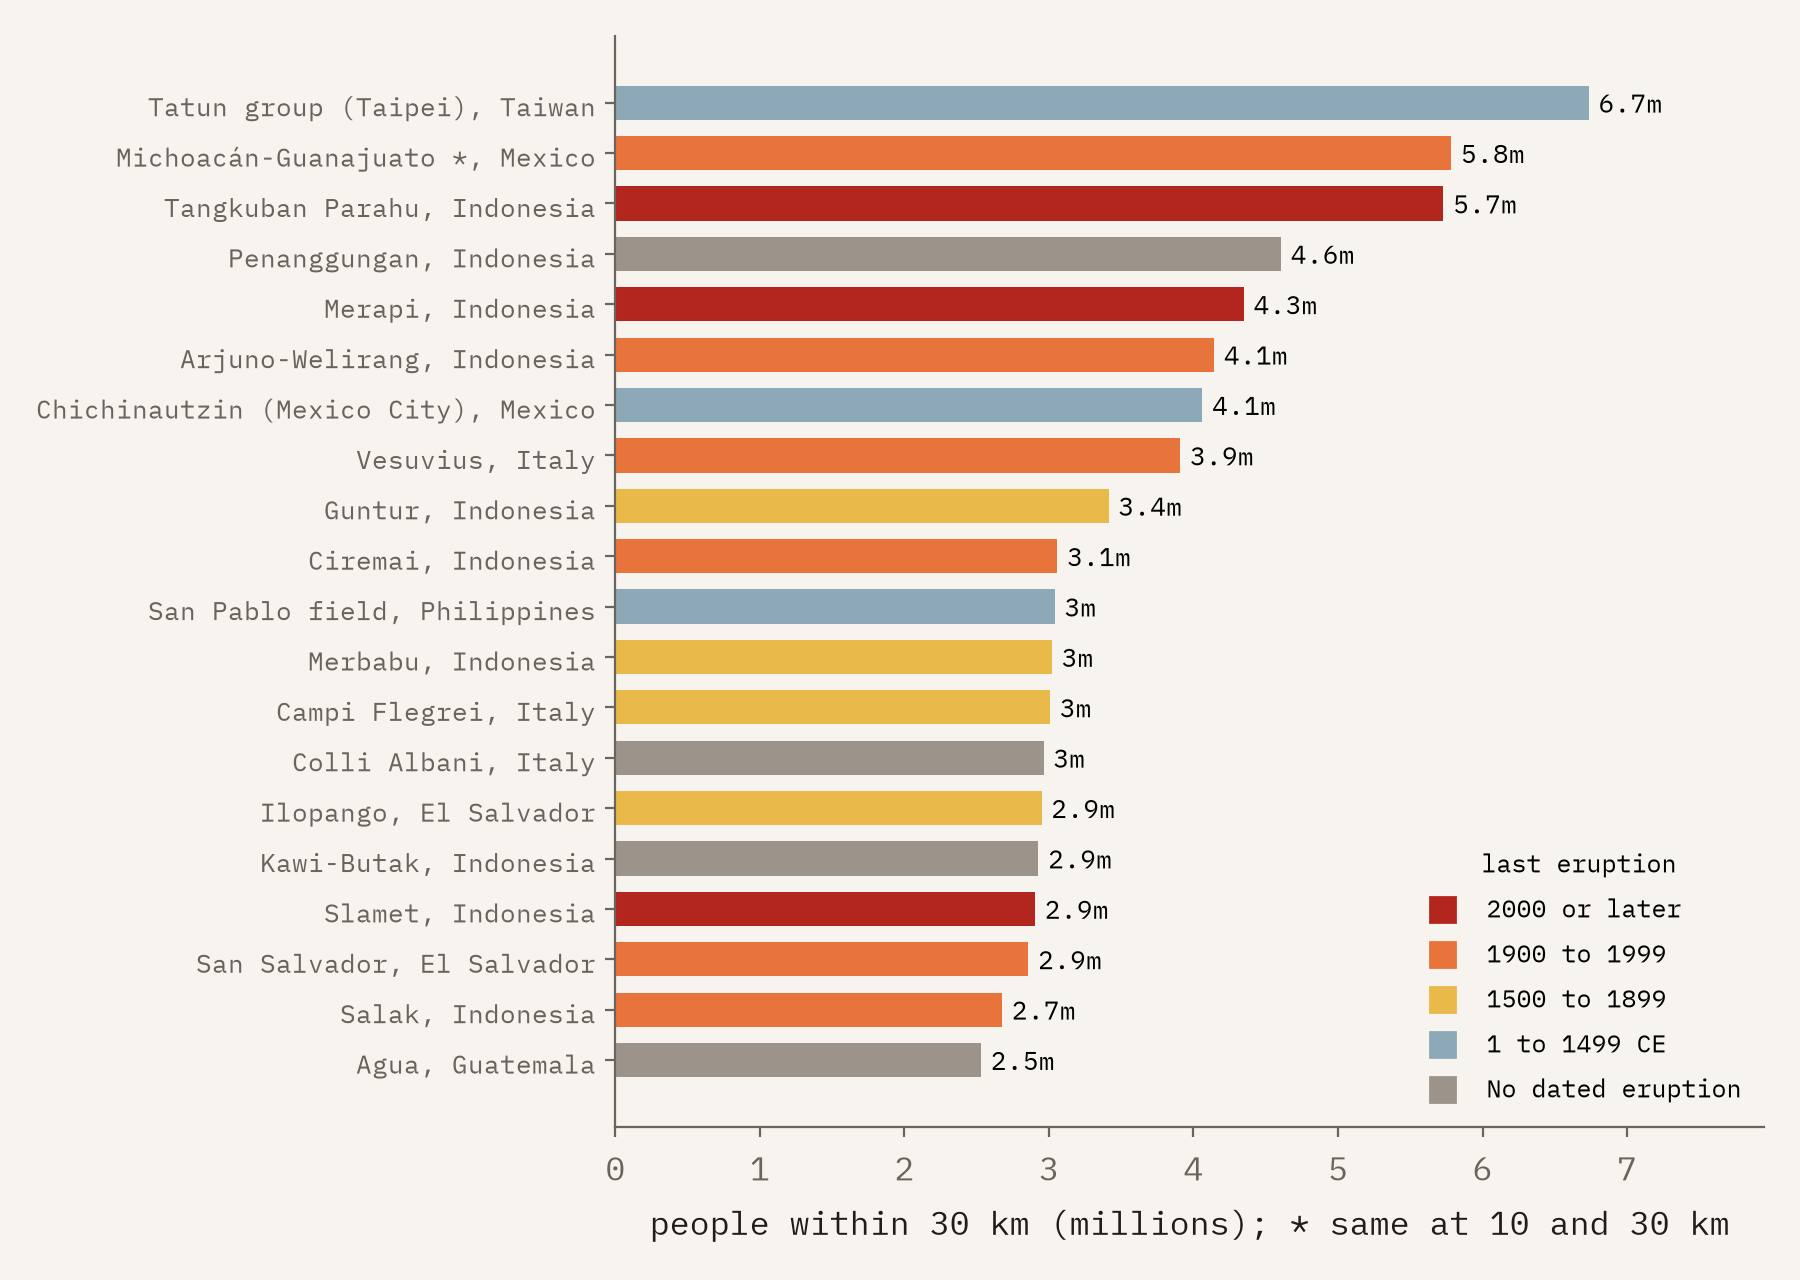
\includegraphics[width=.86\textwidth]{f_top30.png}
\caption{The twenty volcanoes with most people within 30 km, coloured by last known eruption. An asterisk marks a volcano with the same figure at 10 and 30 km.}\label{fig:top}\end{figure}

\begin{table}[tbp]\centering\small\caption{The twenty volcanoes with most people within 30 km (GVP names and figures). $^*$ same figure at 10 and 30 km.}\label{tab:top}\setlength{\tabcolsep}{4pt}\begin{tabular}{lllrrr}\toprule Volcano & Country & Last eruption & Within 10 km & Within 30 km & Within 100 km\\\midrule
Tatun Volcanic Group & Taiwan & 648 CE & 5,084,149 & 6,735,396 & 9,862,061\\
Michoacan-Guanajuato$^*$ & Mexico & 1952 CE & 5,783,287 & 5,783,287 & 5,783,287\\
Tangkuban Parahu & Indonesia & 2019 CE & 518,822 & 5,729,309 & 32,855,731\\
Penanggungan & Indonesia & Unknown & 416,275 & 4,605,710 & 25,773,159\\
Merapi & Indonesia & 2026 CE & 185,849 & 4,348,473 & 24,728,414\\
Arjuno-Welirang & Indonesia & 1952 CE & 53,983 & 4,143,137 & 25,385,433\\
Chichinautzin & Mexico & 399 CE & 584,725 & 4,061,942 & 28,030,794\\
Vesuvius & Italy & 1944 CE & 675,705 & 3,907,941 & 6,009,961\\
Guntur & Indonesia & 1847 CE & 218,012 & 3,412,038 & 24,486,191\\
Ciremai & Indonesia & 1951 CE & 67,377 & 3,058,015 & 25,718,820\\
San Pablo Volcanic Field & Philippines & 1350 CE & 1,349,742 & 3,039,334 & 24,626,975\\
Merbabu & Indonesia & 1797 CE & 249,747 & 3,019,783 & 25,096,234\\
Campi Flegrei & Italy & 1538 CE & 2,234,109 & 3,006,865 & 6,019,697\\
Colli Albani & Italy & Unknown & 897,039 & 2,962,194 & 5,330,273\\
Ilopango & El Salvador & 1880 CE & 2,049,583 & 2,948,989 & 6,689,160\\
Kawi-Butak & Indonesia & Unknown & 127,978 & 2,927,446 & 24,141,573\\
Slamet & Indonesia & 2014 CE & 13,401 & 2,904,026 & 20,217,467\\
San Salvador & El Salvador & 1917 CE & 800,780 & 2,857,563 & 6,366,833\\
Salak & Indonesia & 1938 CE & 80,578 & 2,675,904 & 38,154,252\\
Agua & Guatemala & Unknown & 114,404 & 2,530,449 & 7,441,660\\
\bottomrule\end{tabular}\end{table}

\begin{figure}[tbp]\centering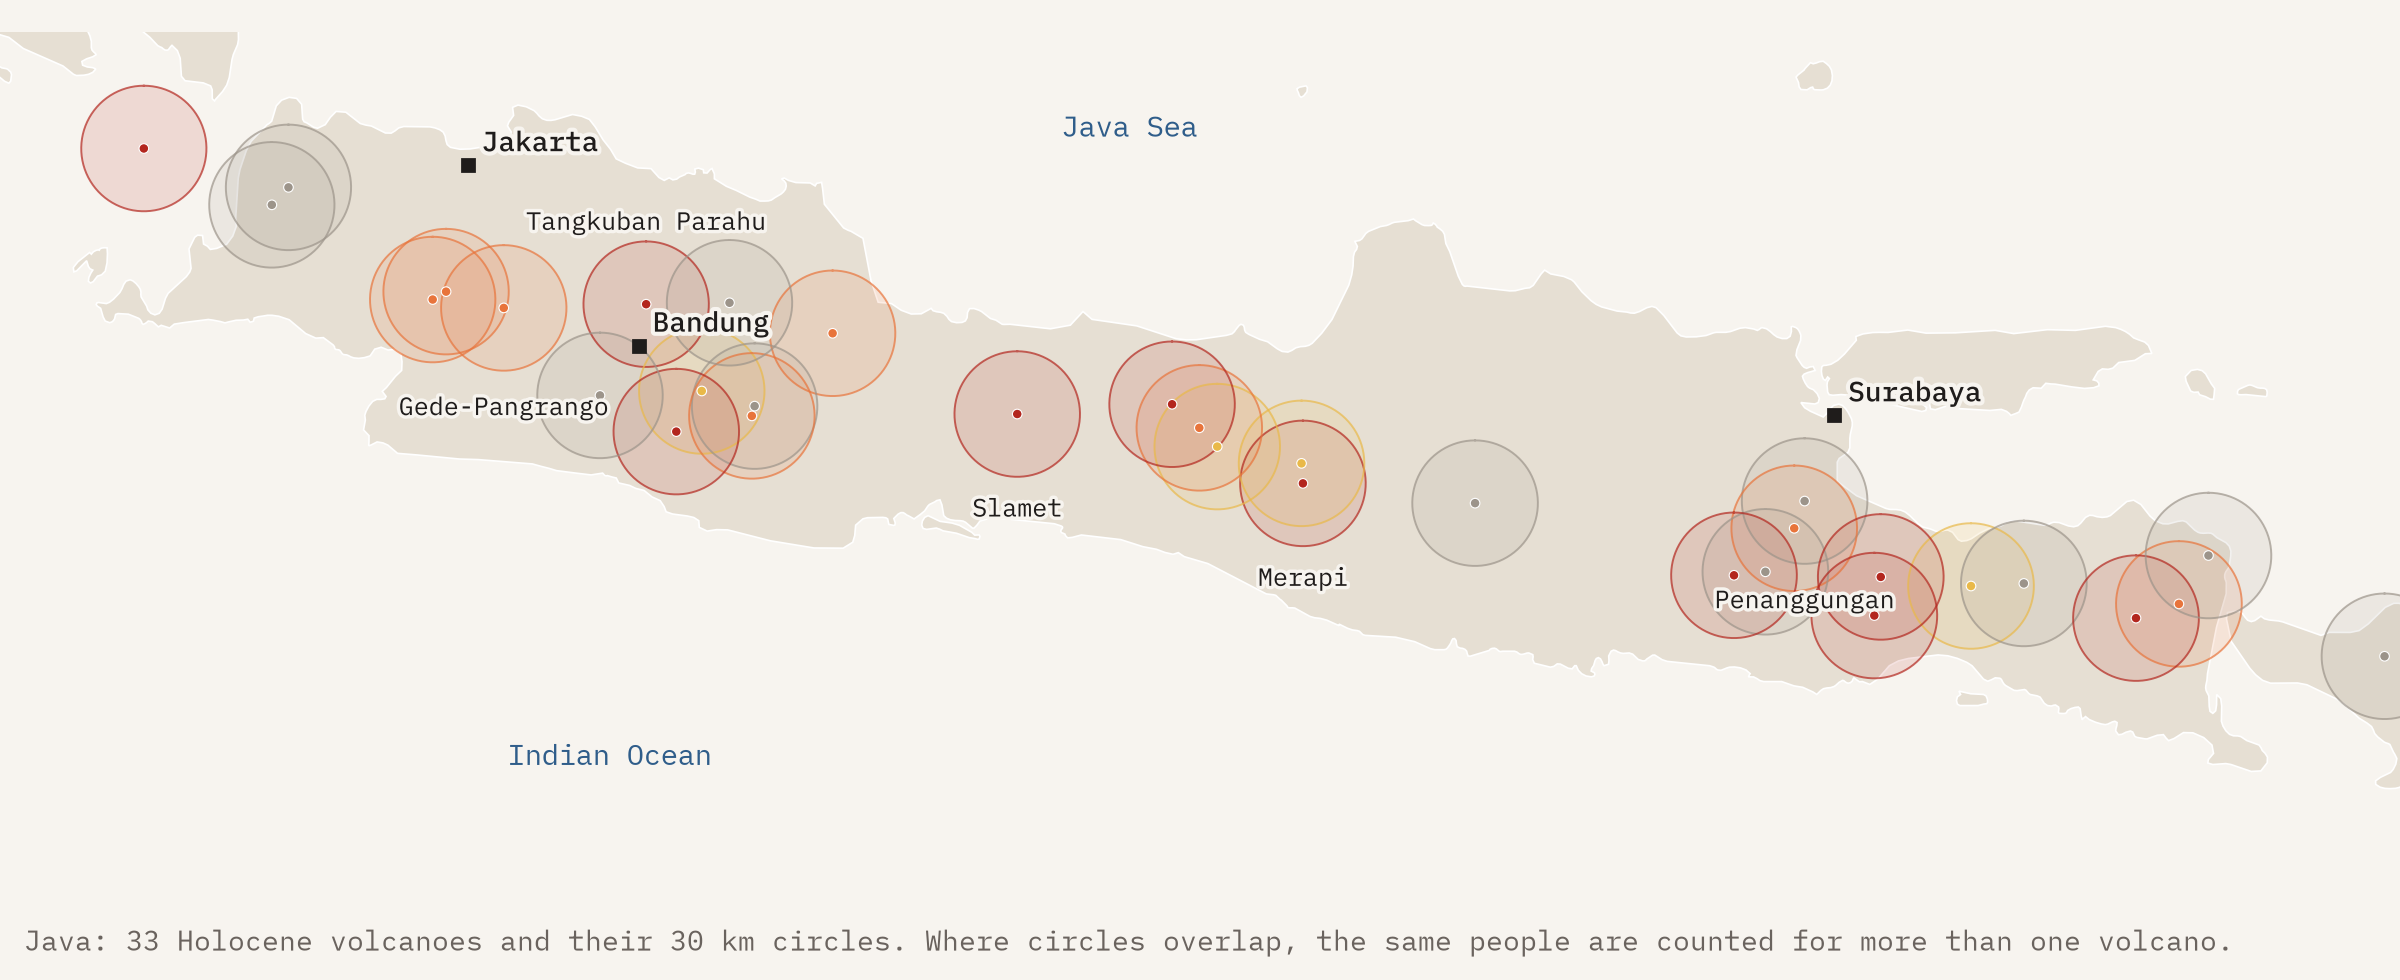
\includegraphics[width=\textwidth]{f_java.png}
\caption{Java's Holocene volcanoes and their 30 km circles, coloured by last eruption. Overlapping circles are why the simple sum overstates the number of people.}\label{fig:java}\end{figure}

\subsection{Recent eruptions near people}
231 volcanoes have erupted since 2000 and 207 last erupted in the twentieth century. At least 84.4 million people live within 30 km of a volcano that has erupted since 1900, and at least 55.0 million within 30 km of one that has erupted since 2000 (Figure~\ref{fig:ecls}). 21 volcanoes that have erupted since 2000 have a million or more people within 30 km; the most crowded are Tangkuban Parahu (last eruption 2019), Merapi, Slamet, Pacaya and Taal (Figure~\ref{fig:recent}). Eruptions that began in 2025 or 2026, the last years in the list, came from 30 volcanoes with 5,137,145 people within 30 km between them, led by Mayon (1,166,441). Volcanoes with no dated eruption are not empty: at least 47.3 million people live within 30 km of one, a reminder that a volcano without a historical eruption is not necessarily extinct.

\begin{figure}[tbp]\centering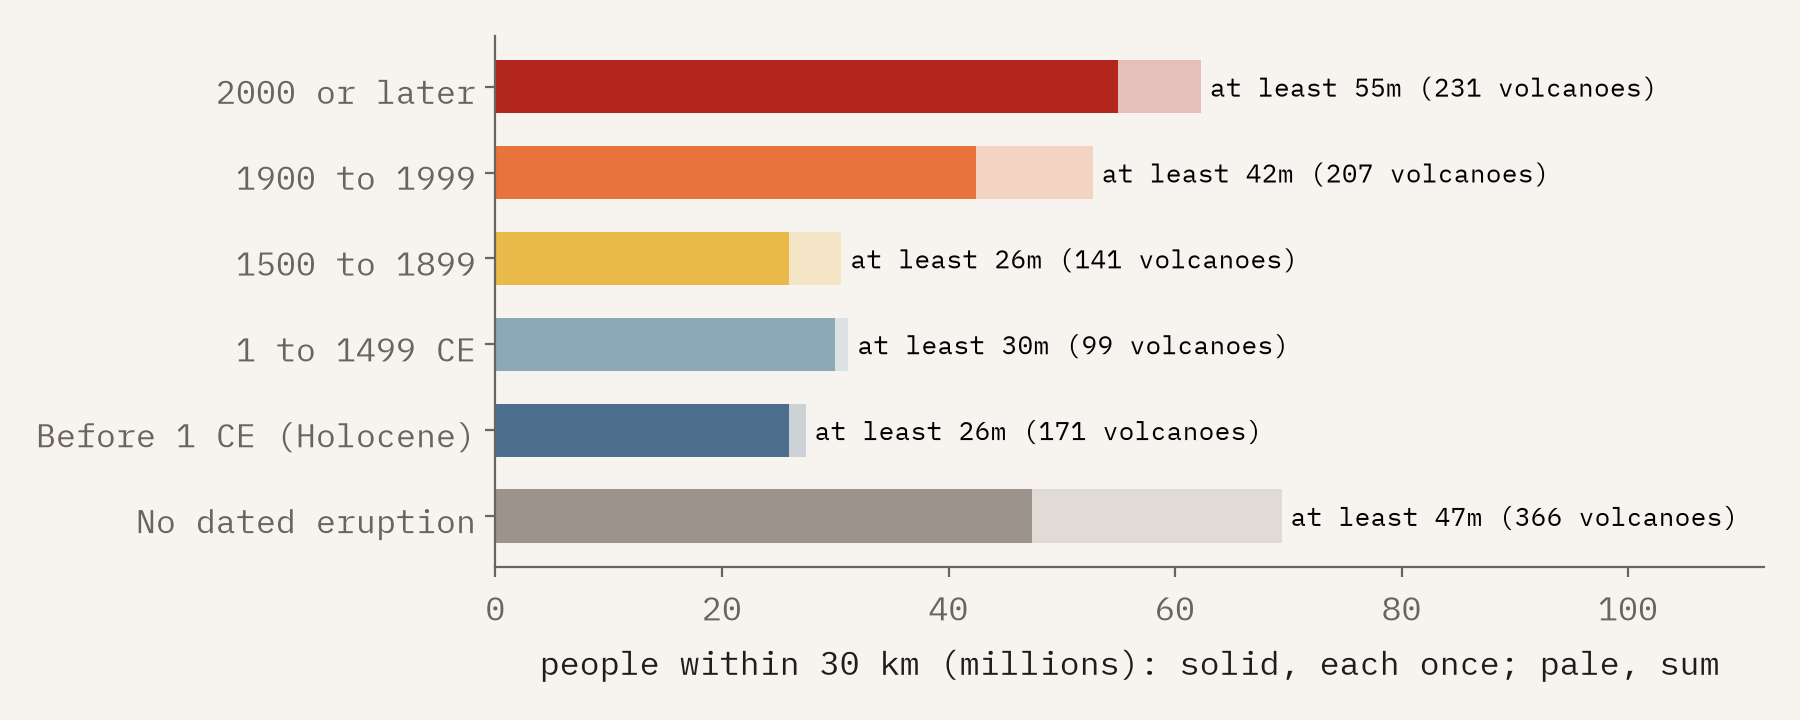
\includegraphics[width=.86\textwidth]{f_ecls.png}
\caption{People within 30 km of volcanoes grouped by last known eruption: lower bound (solid) and simple sum (pale).}\label{fig:ecls}\end{figure}

\begin{figure}[tbp]\centering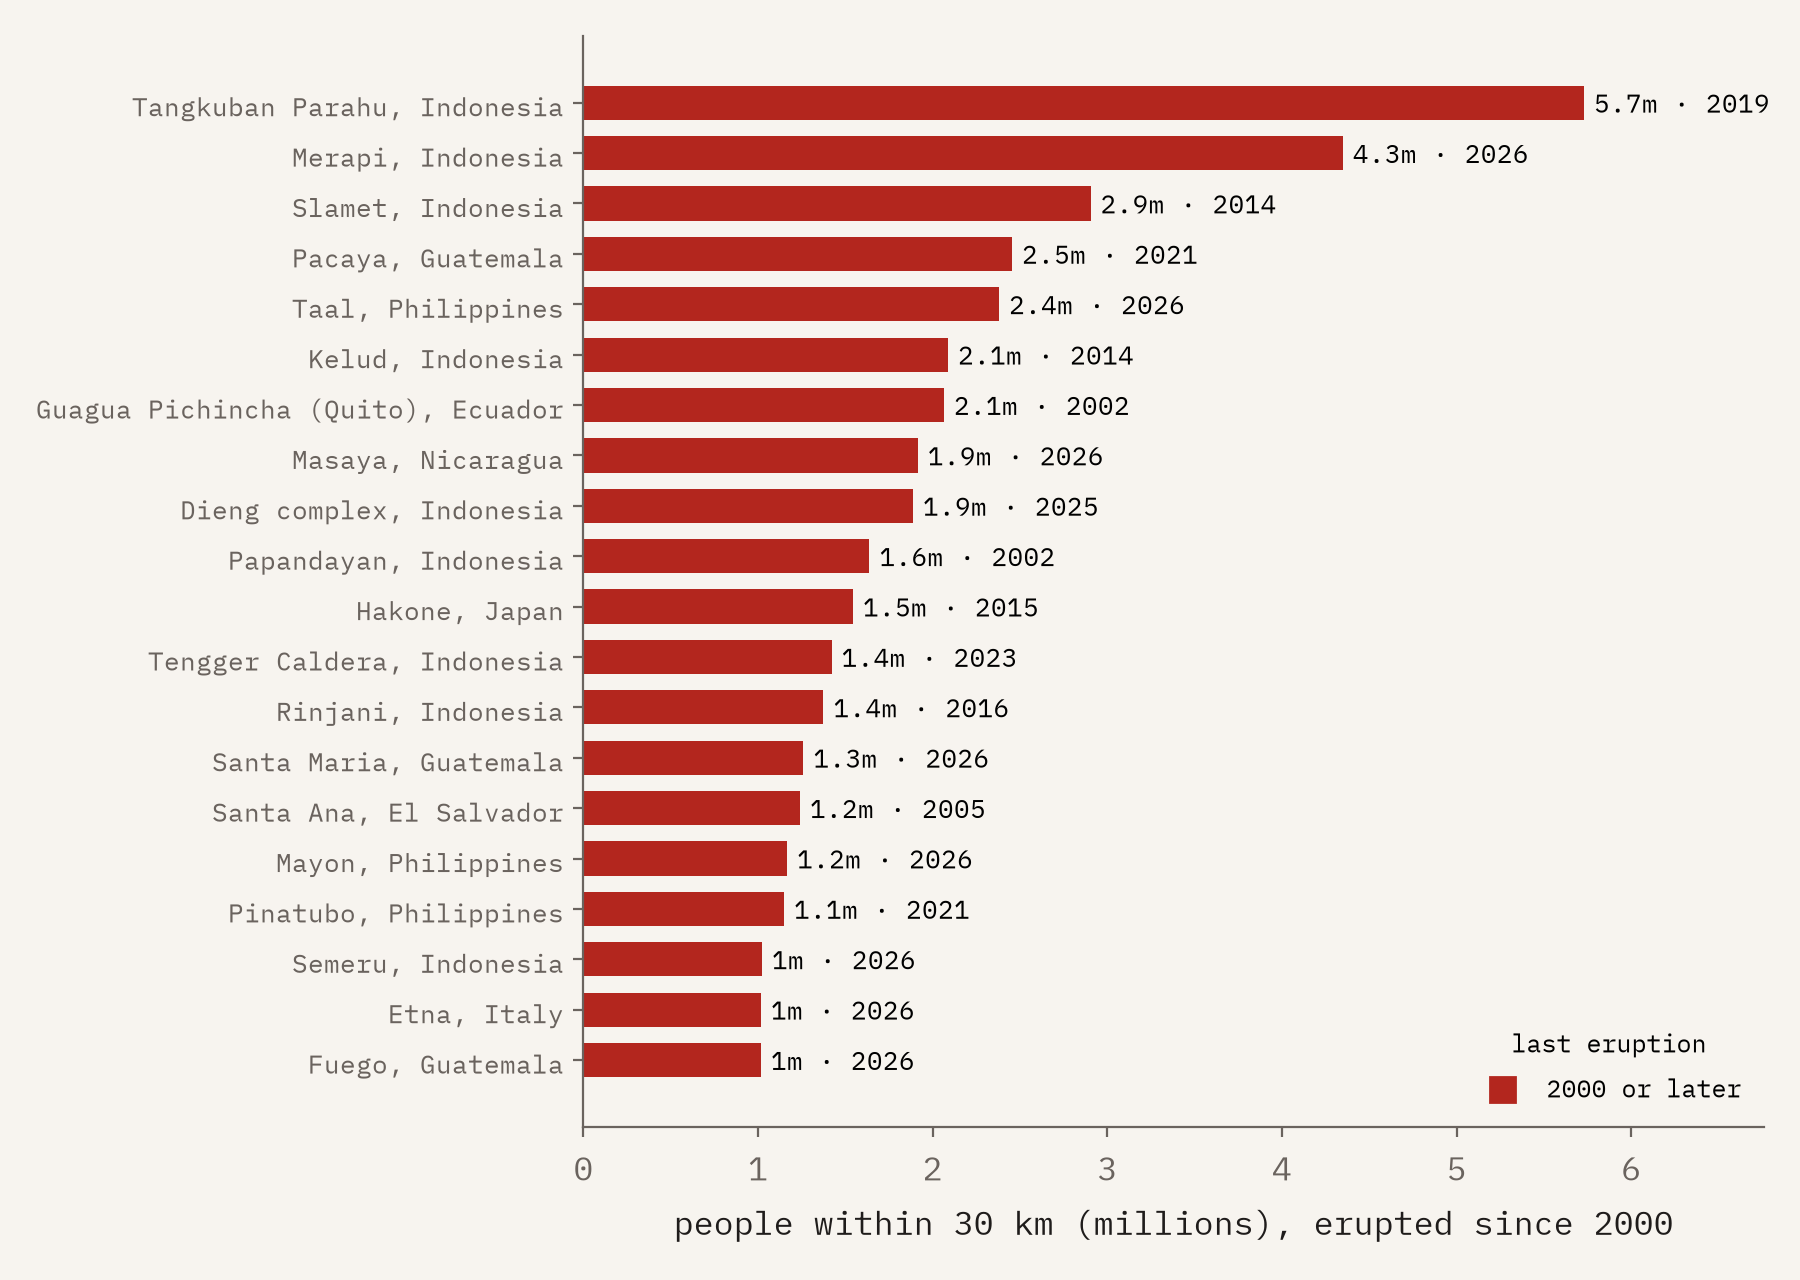
\includegraphics[width=.86\textwidth]{f_recent.png}
\caption{The twenty volcanoes that have erupted since 2000 with most people within 30 km, with the year of the last known eruption.}\label{fig:recent}\end{figure}

\subsection{Eruptions through time and reporting bias}
The eruption list grows steeply towards the present (Figure~\ref{fig:cent}): 247 confirmed eruptions started in the sixteenth century, 337 in the seventeenth, 499 in the eighteenth, 1,502 in the nineteenth and 2,957 in the twentieth; 947 started between 2000 and 2026, about 35 a year against 30 a year in the twentieth century. 55\% of all Holocene eruptions in the list started in 1800 or later. This is the familiar signature of under-recording in the past \citep{simkin1993,deligne2010}: 64\% of eruptions are dated by reported observation, so the record depends on people being present to see, and later on instruments and satellites. Eruptions of VEI 4 or more, which leave widespread deposits that can be dated long afterwards, are recorded much more evenly: their number rises 2.0-fold from the seventeenth to the twentieth century, compared with 8.8-fold for all eruptions. 193 volcanoes have no eruption in the list before 1800. The rising curve should not be read as a rise in volcanic activity.

\begin{figure}[tbp]\centering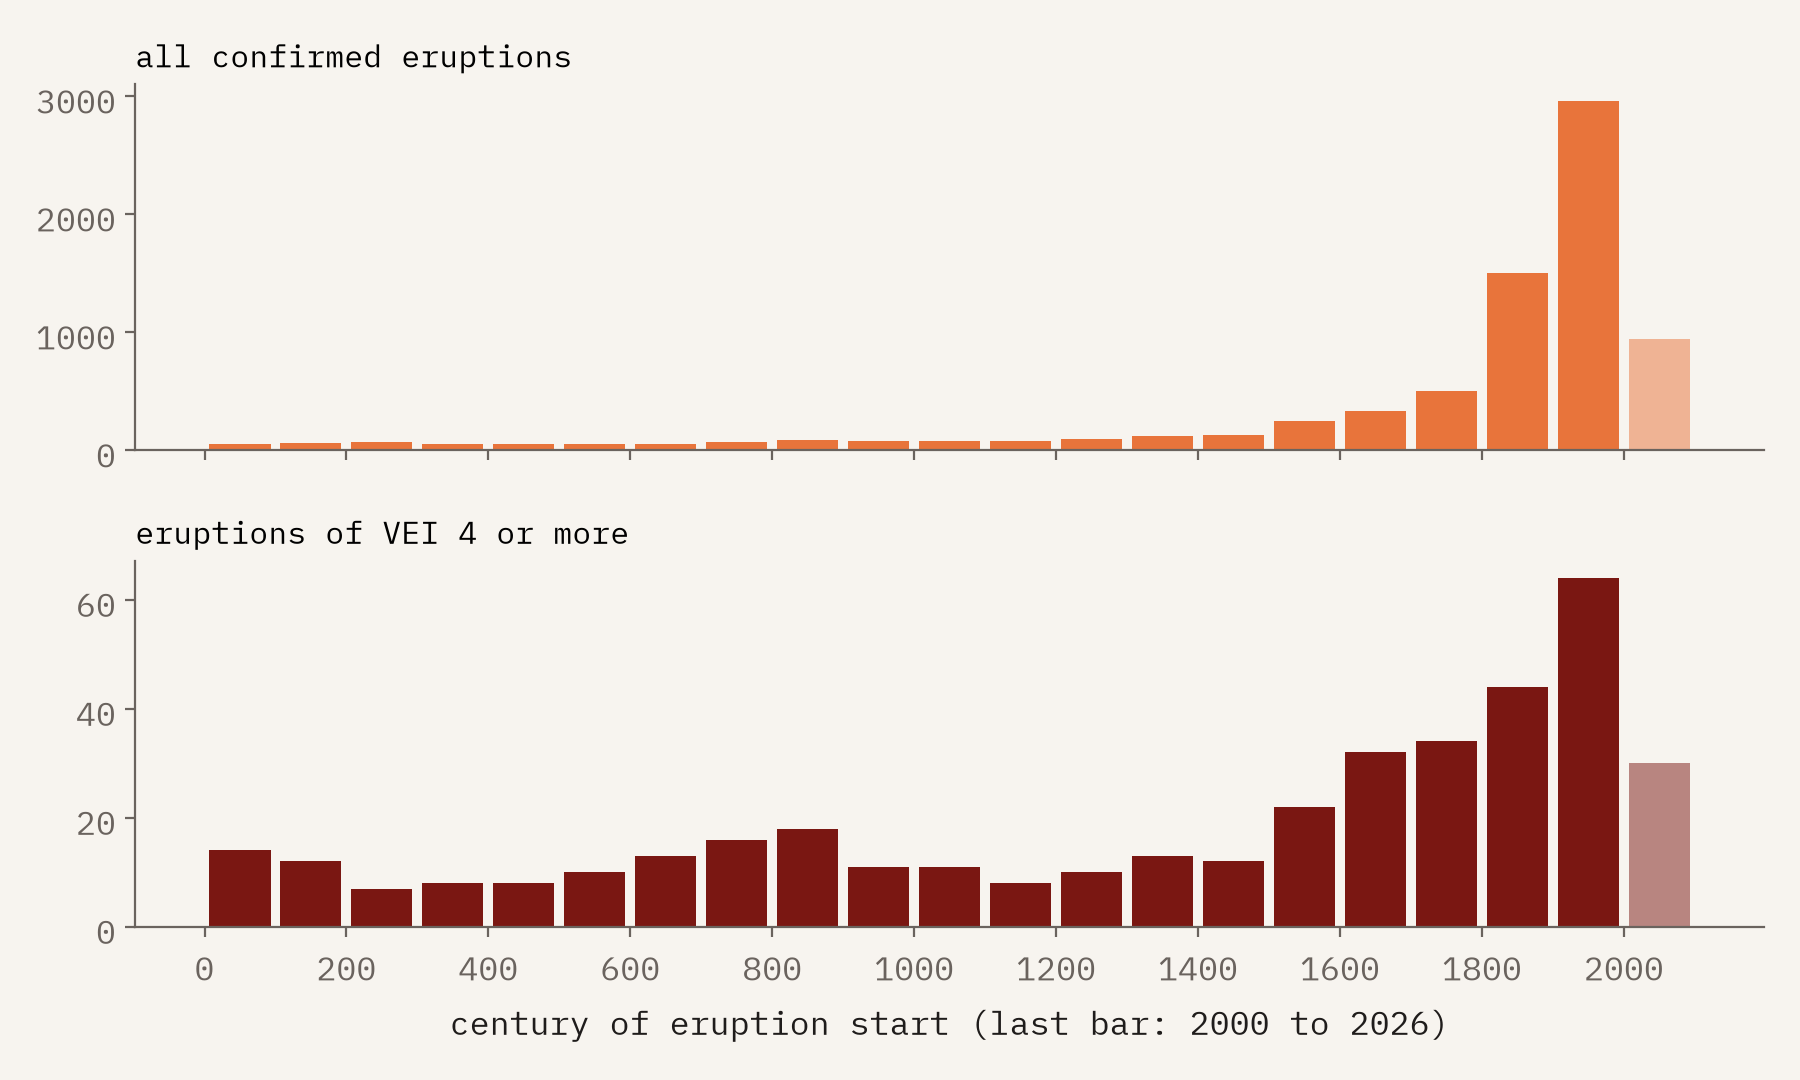
\includegraphics[width=.86\textwidth]{f_centuries.png}
\caption{Confirmed eruptions per century of start, 1 CE to 2026: all eruptions (top) and eruptions of VEI 4 or more (bottom). The last bar covers 2000 to 2026 only.}\label{fig:cent}\end{figure}

\subsection{Deaths}
The NCEI database lists 442 eruptions with deaths recorded between 141 BCE and 2024, with 286,065 deaths in total, of which 92,042 were in eruptions since 1900. The deadliest are Tambora in 1815 (60,000), Krakatau in 1883 (36,417), Ilopango around 450 CE (30,000), Mont Pel\'ee in 1902 (28,000) and Nevado del Ruiz in 1985 (23,080). Several of the deadliest volcanoes have few people near them today (Tambora has 89,006 within 30 km), while Ilopango, now on the edge of San Salvador, has 2,948,989.

\section{Discussion}
Three points stand out. First, the number of people near volcanoes depends heavily on how overlap is handled. Within 10 km it hardly matters; within 100 km a simple sum overstates the true figure several times. Studies that report sums of per-volcano figures should say so, and the bounds here give a cheap check when no population grid is at hand. Second, exposure is concentrated: a small number of countries, led by Indonesia, and a few dozen volcanoes, many in Java, account for most of it. Third, the volcanoes nearest the most people are a mix of very active ones, such as Merapi and Taal, and ones with no historical eruption at all, such as Penanggungan; the GVP's list is a list of volcanoes that could erupt, not only of those that have.

\section{Limitations}
First, distance is not hazard: the area affected by an eruption depends on its size and style, the shape of the land, the wind and river systems, and the GVP's listed point is a single location for what may be a large field. Second, the population figures are a fixed snapshot of unstated date and source and are joined from an older version of the database; 6 volcanoes lack them, and for 16 the figures are the same at 10 and 30 km. Third, the lower bound uses a greedy choice of non-overlapping circles and can be well below the true figure at 100 km. Fourth, country totals include people across borders. Fifth, the eruption record is incomplete in the past, as shown above, and the death figures for early eruptions are rough estimates. Finally, the volcano and eruption lists were taken from copies posted to GitHub and identified by their headers, not downloaded directly by me.

\section{Conclusion}
At least 52.9 million people live within 10 km and at least 147.5 million within 30 km of a volcano that has been active in the Holocene, most of them in Indonesia, Mexico, Japan, the Philippines, Italy, Taiwan and Central America. The interactive map lets readers find any volcano, see its 10, 30 and 100 km rings and compare its neighbours with its eruption history.

\section*{Data and code availability}
The interactive map is at \url{https://maps.tristanhotham.com/volcano-neighbours/}. Data and code are at \url{https://github.com/Tristan-Hotham/volcano-neighbours} and archived with this paper at \url{https://doi.org/10.5281/zenodo.23847550}. Inputs: the GVP Holocene volcano list, version 5.3.5 (copy at \url{https://github.com/bciupak/Wizualizacja-Danych-Projekty}), the GVP Holocene eruption list, version 5.3.5 (copy at \url{https://github.com/im-hana-s/ML-mini-project}), and the GVP volcano list with population columns, version 5.1.7 (copy at \url{https://github.com/Matteo2979/Volcano-Analysis}, which also holds the NCEI table). GVP data are used under the Smithsonian's terms of use (non-commercial use with credit), and the derived tables keep those terms. The text and figures are released under CC BY 4.0 and the code under the MIT licence.

\section*{AI statement}
I wrote the text, with drafting and editing assistance from Claude (Anthropic), which also helped prepare the analysis code. I reviewed and checked all text and results.

\begin{thebibliography}{9}
\bibitem[Bird(2003)]{bird2003} Bird, P. (2003) An updated digital model of plate boundaries. \emph{Geochemistry, Geophysics, Geosystems}, 4(3), 1027. GeoJSON by H. Ahlenius, Nordpil, Open Data Commons Attribution License 1.0.
\bibitem[Brown et~al.(2015)]{brown2015} Brown, S.K., Auker, M.R. and Sparks, R.S.J. (2015) Populations around Holocene volcanoes and development of a Population Exposure Index. In Loughlin, S.C., Sparks, R.S.J., Brown, S.K., Jenkins, S.F. and Vye-Brown, C. (eds) \emph{Global Volcanic Hazards and Risk}. Cambridge: Cambridge University Press, 223 to 232.
\bibitem[Deligne et~al.(2010)]{deligne2010} Deligne, N., Coles, S. and Sparks, R.S.J. (2010) Recurrence rates of large explosive volcanic eruptions. \emph{Journal of Geophysical Research}, 115, B06203.
\bibitem[GVP(2024)]{gvp517} Global Volcanism Program (2024) Volcanoes of the World (v. 5.1.7). Distributed by Smithsonian Institution, compiled by Venzke, E. \url{https://volcano.si.edu/} (accessed via the named GitHub mirrors).
\bibitem[GVP(2025)]{gvp535} Global Volcanism Program (2025) Volcanoes of the World (v. 5.3.5). Distributed by Smithsonian Institution, compiled by Venzke, E. \url{https://volcano.si.edu/} (accessed via the named GitHub mirrors).
\bibitem[Natural Earth(2026)]{naturalearth} Natural Earth (2026) Admin 0 countries and populated places. Public domain. \url{https://www.naturalearthdata.com/}
\bibitem[NCEI(2024)]{ncei} National Geophysical Data Center / World Data Service (NGDC/WDS) NCEI/WDS Global Significant Volcanic Eruptions Database. NOAA National Centers for Environmental Information. doi:10.7289/V5JW8BSH.
\bibitem[Newhall and Self(1982)]{newhall1982} Newhall, C.G. and Self, S. (1982) The volcanic explosivity index (VEI): an estimate of explosive magnitude for historical volcanism. \emph{Journal of Geophysical Research}, 87(C2), 1231 to 1238.
\bibitem[Simkin and Siebert(1994)]{simkin1993} Simkin, T. and Siebert, L. (1994) \emph{Volcanoes of the World}, 2nd edition. Tucson: Geoscience Press and Smithsonian Institution.
\end{thebibliography}
\end{document}
